\documentclass[12pt,a4paper]{article}

% ─── Page Layout ───────────────────────────────────────────────────────────────
\usepackage[a4paper, margin=0.8in, headheight=14pt]{geometry}

% ─── Fonts (XeLaTeX) ───────────────────────────────────────────────────────────
\usepackage{fontspec}
\usepackage{unicode-math}
\setmainfont{TeX Gyre Pagella}
\setmonofont[Scale=0.88]{TeX Gyre Cursor}
\setmathfont{Latin Modern Math}

% ─── Packages ──────────────────────────────────────────────────────────────────
\usepackage{xcolor}
\usepackage{colortbl}
\usepackage{titlesec}
\usepackage{enumitem}
\usepackage{tabularx}
\usepackage{booktabs}
\usepackage{array}
\usepackage{amsmath}
\usepackage{tikz}
\usetikzlibrary{shapes.geometric, arrows.meta, positioning, calc, fit, decorations.pathreplacing, decorations.pathmorphing}
\usepackage{tcolorbox}
\tcbuselibrary{skins, breakable}
\usepackage{hyperref}
\usepackage{fancyhdr}
\usepackage{graphicx}
\usepackage{microtype}
\hyphenpenalty=10000
\exhyphenpenalty=10000
\sloppy
\usepackage{caption}
\usepackage{setspace}
\usepackage{multirow}
\usepackage{tocloft}

% ─── Q&A helper ────────────────────────────────────────────────────────────────
\newcommand{\Q}[1]{\textbf{#1}\par\noindent\ignorespaces}

% ─── Colour Palette ────────────────────────────────────────────────────────────
\definecolor{myred}{RGB}{196,30,58}
\definecolor{mydark}{RGB}{30,30,50}
\definecolor{mygreen}{RGB}{14,120,80}
\definecolor{myteal}{RGB}{0,130,140}
\definecolor{myamber}{RGB}{180,100,0}
\definecolor{mypurple}{RGB}{100,30,160}
\definecolor{mygray}{RGB}{246,247,249}
\definecolor{mgframe}{RGB}{180,185,200}
\definecolor{watermark}{RGB}{145,150,170}
\definecolor{hdrred}{RGB}{250,232,235}
\definecolor{hdrgreen}{RGB}{220,244,233}
\definecolor{hdrteal}{RGB}{220,242,244}
\definecolor{hdramber}{RGB}{253,242,215}
\definecolor{hdrpurple}{RGB}{238,228,255}
\definecolor{hdrgray}{RGB}{238,240,245}
\definecolor{rowalt}{RGB}{250,251,253}

% ─── Section Formatting ────────────────────────────────────────────────────────
\titleformat{\section}
  {\large\bfseries\color{myred}}{\thesection.}{0.5em}{}
  [\vspace{1pt}{\color{myred}\rule{\linewidth}{0.8pt}}]
\titleformat{\subsection}
  {\normalsize\bfseries\color{myteal}}{\thesubsection}{0.5em}{}
\titlespacing*{\section}{0pt}{18pt}{7pt}
\titlespacing*{\subsection}{0pt}{11pt}{4pt}

% ─── Paragraph ─────────────────────────────────────────────────────────────────
\setlength{\parindent}{0pt}
\setlength{\parskip}{4pt}

% ─── TOC Styling ───────────────────────────────────────────────────────────────
\renewcommand{\cfttoctitlefont}{\large\bfseries\color{myred}}
\renewcommand{\cftaftertoctitle}{\par\noindent{\color{myred}\rule{\linewidth}{0.8pt}}}
\setlength{\cftbeforetoctitleskip}{0pt}
\setlength{\cftaftertoctitleskip}{6pt}
\renewcommand{\cftsecfont}{\normalsize\bfseries\color{mydark}}
\renewcommand{\cftsecpagefont}{\normalsize\bfseries\color{mydark}}
\renewcommand{\cftsecleader}{\cftdotfill{\cftdotsep}}
\setlength{\cftbeforesecskip}{7pt}
\renewcommand{\cftsubsecfont}{\small\color{mydark}}
\renewcommand{\cftsubsecpagefont}{\small\color{mydark}}
\setlength{\cftbeforesubsecskip}{3pt}
\setlength{\cftsubsecindent}{1.4em}

% ─── Table helpers ─────────────────────────────────────────────────────────────
\renewcommand{\arraystretch}{1.45}
\setlength{\tabcolsep}{6pt}
\arrayrulecolor{mydark}
\newcolumntype{B}[1]{>{\small\bfseries\raggedright\arraybackslash}m{#1}}
\newcolumntype{C}[1]{>{\centering\arraybackslash}m{#1}}
\newcolumntype{Y}{>{\small\raggedright\arraybackslash}X}
\renewcommand{\tabularxcolumn}[1]{m{#1}}

% ─── Header / Footer ───────────────────────────────────────────────────────────
\pagestyle{fancy}
\fancyhf{}
\fancyhead[L]{\small\color{myred}\textbf{OE-EC704A}\;\color{mydark}--- Web Technology}
\fancyhead[R]{\small\color{myteal}\textbf{Module 9 Notes}}
\fancyfoot[C]{\small\color{mydark}\thepage}
\fancyfoot[R]{\small\color{watermark}\textit{\copyright\ Biraj}}
\renewcommand{\headrulewidth}{0.5pt}
\renewcommand{\footrulewidth}{0.3pt}

% ─── Hyperref ──────────────────────────────────────────────────────────────────
\hypersetup{
  colorlinks=true, linkcolor=myteal, urlcolor=myteal,
  pdfauthor={Biraj Sarkar},
  pdftitle={OE-EC704A --- Module 9 Notes}
}

% ─── tcolorbox styles ──────────────────────────────────────────────────────────
\tcbset{
  tikzbox/.style={
    colback=mygray, colframe=mgframe, boxrule=0.6pt, arc=4pt,
    left=8pt, right=8pt, top=6pt, bottom=6pt,
    colbacktitle=mgframe, coltitle=mydark,
    fonttitle=\small\bfseries
  },
  defbox/.style={
    colback=hdrgreen, colframe=mygreen, boxrule=0.8pt, arc=4pt,
    left=9pt, right=9pt, top=6pt, bottom=6pt,
    colbacktitle=mygreen, coltitle=white,
    fonttitle=\small\bfseries
  },
  formulabox/.style={
    colback=hdrteal, colframe=myteal, boxrule=0.8pt, arc=4pt,
    left=9pt, right=9pt, top=7pt, bottom=7pt,
    colbacktitle=myteal, coltitle=white,
    fonttitle=\small\bfseries
  },
  examplebox/.style={
    colback=hdramber, colframe=myamber, boxrule=0.8pt, arc=4pt,
    left=9pt, right=9pt, top=6pt, bottom=6pt,
    colbacktitle=myamber, coltitle=white,
    fonttitle=\small\bfseries
  },
  masonbox/.style={
    colback=hdrpurple, colframe=mypurple, boxrule=0.8pt, arc=4pt,
    left=9pt, right=9pt, top=6pt, bottom=6pt,
    colbacktitle=mypurple, coltitle=white,
    fonttitle=\small\bfseries
  },
  exambox/.style={
    colback=hdrpurple, colframe=mypurple, boxrule=1pt, arc=5pt,
    left=10pt, right=10pt, top=8pt, bottom=8pt,
    colbacktitle=mypurple, coltitle=white,
    fonttitle=\bfseries,
    breakable, title after break={\textbf{Frequently Asked / Viva Questions (contd.)}}}
}
\tcbset{breakable}

% ─── TikZ styles ───────────────────────────────────────────────────────────────
\tikzset{
  block/.style={rectangle, draw=myteal, fill=hdrteal,
    text width=2.5cm, align=center, minimum height=1.0cm,
    font=\small, rounded corners=3pt, line width=0.7pt},
  redblock/.style={rectangle, draw=myred, fill=hdrred,
    text width=2.5cm, align=center, minimum height=1.0cm,
    font=\small, rounded corners=3pt, line width=0.7pt},
  netnode/.style={rectangle, draw=myteal, fill=hdrteal,
    text width=1.8cm, align=center, minimum height=0.8cm,
    font=\small, rounded corners=3pt, line width=0.7pt},
  sumjunc/.style={circle, draw=myamber, fill=hdramber,
    minimum size=0.6cm, font=\small, line width=0.8pt},
  snode/.style={circle, draw=mypurple, fill=hdrpurple,
    minimum size=0.55cm, font=\footnotesize, line width=0.7pt},
  arrow/.style={-Stealth, thick, color=mydark},
  redarrow/.style={-Stealth, thick, color=myred},
  line/.style={thick, color=mydark}
}

% ═══════════════════════════════════════════════════════════════════════════════
\begin{document}
% ═══════════════════════════════════════════════════════════════════════════════

\begin{center}
  {\LARGE\bfseries\color{myred} OE-EC704A --- Web Technology}\\[5pt]
  {\normalsize\color{mydark} Semester VII \quad$\bullet$\quad 3L:0T:0P \quad$\bullet$\quad 3 Credits}\\[3pt]
  {\normalsize\color{myteal}\textbf{Module 9 Exam Notes: Java Applets}}\\[3pt]
  {\small\color{mydark} CGEC \;$|$\; B.Tech ECE (2023--27) \;$|$\; \textit{Biraj Sarkar}}
\end{center}
\noindent{\color{myred}\rule{\linewidth}{1.5pt}}
\vspace{2pt}

\hypersetup{linkcolor=mydark}
\tableofcontents
\hypersetup{linkcolor=myteal}
\newpage

% ===============================================================================
\section{Introduction to Applets}
% ===============================================================================

An applet is a specialized Java program designed to be embedded within an HTML web page and executed on a client machine inside a web browser sandbox.

\begin{tcolorbox}[defbox, title={\textbf{Applet Security Sandbox}}]
To prevent malicious code execution on client machines, applets run under strict security constraints:
\begin{itemize}[leftmargin=*, itemsep=3pt]
  \item Applets cannot read or write files on the local client disk.
  \item Applets cannot communicate with any host except the one they were downloaded from.
  \item Applets cannot execute local system commands or load native runtime libraries.
\end{itemize}
\end{tcolorbox}

\subsection{Applet Lifecycle \& Execution}
An applet inherits from \texttt{java.applet.Applet} and does not contain a \texttt{main()} method. Instead, its execution is controlled by the browser or the Java Applet Viewer tool through five lifecycle callback methods:
\begin{itemize}[leftmargin=*, itemsep=4pt]
  \item \textbf{\texttt{init()}:} Invoked once when the applet is first loaded to perform initialization (e.g., setting up GUI components, reading parameters).
  \item \textbf{\texttt{start()}:} Invoked after \texttt{init()} or whenever the user returns to the web page containing the applet. Used to start or resume execution threads.
  \item \textbf{\texttt{paint(Graphics g)}:} Invoked when the applet window needs to be redrawn (e.g., first display, resizing, or revealing). It uses the \texttt{java.awt.Graphics} object.
  \item \textbf{\texttt{stop()}:} Invoked when the user navigates away from the page, pausing background threads to save CPU cycles.
  \item \textbf{\texttt{destroy()}:} Invoked once before unloading the applet completely to free up system resources.
\end{itemize}

\begin{tcolorbox}[tikzbox, title={Applet Life Cycle State Transitions}]
\centering
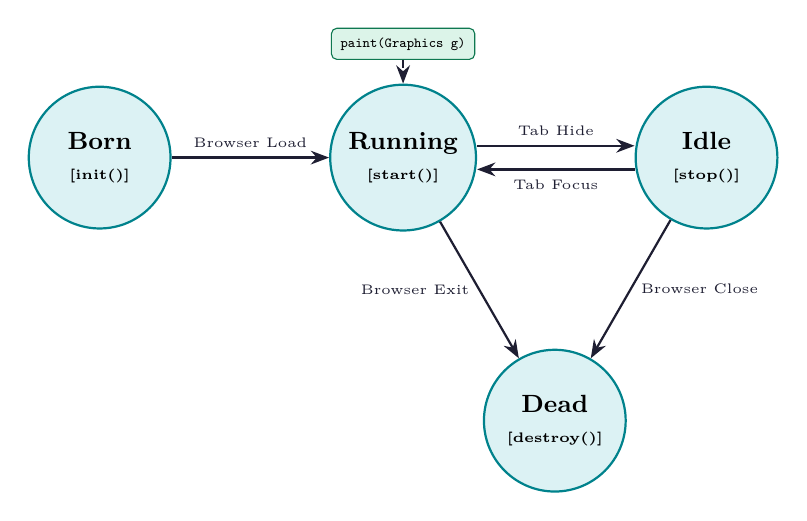
\begin{tikzpicture}[node distance=1.3cm and 2.0cm,
  state/.style={circle, draw=myteal, fill=hdrteal, minimum size=1.8cm,
    align=center, font=\small\bfseries, line width=0.8pt},
  act/.style={rectangle, draw=myamber, fill=hdramber, minimum height=0.6cm,
    font=\tiny, rounded corners=2pt, line width=0.6pt}]

  % States
  \node[state] (born) {Born\\{\tiny [init()]}};
  \node[state, right=2.0cm of born] (run) {Running\\{\tiny [start()]}};
  \node[state, right=2.0cm of run] (idle) {Idle\\{\tiny [stop()]}};
  \node[state, below=1.5cm of $(run.south)!0.5!(idle.south)$] (dead) {Dead\\{\tiny [destroy()]}};

  % Paths
  \draw[arrow] (born) -- (run) node[midway, above, font=\tiny] {Browser Load};
  \draw[arrow, transform canvas={yshift=0.15cm}] (run) -- (idle) node[midway, above, font=\tiny] {Tab Hide};
  \draw[arrow, transform canvas={yshift=-0.15cm}] (idle) -- (run) node[midway, below, font=\tiny] {Tab Focus};
  \draw[arrow] (idle) -- (dead) node[midway, right, font=\tiny] {Browser Close};
  \draw[arrow] (run) -- (dead) node[midway, left, font=\tiny] {Browser Exit};

  % Paint Call
  \node[draw=mygreen, fill=hdrgreen, rounded corners=2pt, above=0.3cm of run, font=\tiny] (pnt) {\texttt{paint(Graphics g)}};
  \draw[arrow, dashed] (pnt) -- (run);
\end{tikzpicture}
\end{tcolorbox}

% ===============================================================================
\section{Applet Display and Status Window}
% ===============================================================================

Since \texttt{Applet} extends the AWT \texttt{Panel} container class, it supports all standard component styling methods:
\begin{itemize}[leftmargin=*, itemsep=3.5pt]
  \item \textbf{\texttt{setBackground(Color c)} / \texttt{setForeground(Color c)}:} Configures the background canvas color and text drawing color.
  \item \textbf{\texttt{showStatus(String msg)}:} Displays the specified text message in the status bar of the browser or Applet Viewer, providing interactive feedback.
\end{itemize}

% ===============================================================================
\section{HTML Embedding and Parameter Passing}
% ===============================================================================

Applets are embedded in web pages using the HTML \texttt{<applet>} tag. 

\subsection{HTML Applet Tag Syntax}
\begin{verbatim}
<applet code="MyApplet.class" width="300" height="200" codebase="bin/">
    <param name="fontName" value="Courier">
    <param name="fontSize" value="14">
    Alt Text: Applets are not supported by your browser.
</applet>
\end{verbatim}
\begin{itemize}[leftmargin=*, itemsep=3pt]
  \item \textbf{\texttt{code}:} Specifies the compiled applet class filename.
  \item \textbf{\texttt{width} \& \texttt{height}:} Declares the size of the applet execution area on the web page.
  \item \textbf{\texttt{codebase}:} Specifies the base directory URL containing the class bytecode.
\end{itemize}

\subsection{Parameter Retrieval via getParameter()}
The \texttt{<param>} tags allow passing configuration parameters to the applet during load time. Inside the applet's \texttt{init()} method, their values are read as Strings:
\begin{verbatim}
String fontStr = getParameter("fontName"); // Returns "Courier"
int size = Integer.parseInt(getParameter("fontSize")); // Parses 14
\end{verbatim}

\subsection{getCodeBase() and getDocumentBase()}
To locate resources (images, audio clips) dynamically:
\begin{itemize}[leftmargin=*, itemsep=3.5pt]
  \item \textbf{\texttt{getCodeBase()}:} Returns the base URL of the directory containing the compiled class bytecode.
  \item \textbf{\texttt{getDocumentBase()}:} Returns the URL of the HTML document embedding the applet.
\end{itemize}

\newpage
% ===============================================================================
\begin{center}
  {\large\bfseries\color{myred} Quick Revision --- Module 9}\\[3pt]
  {\small\color{mydark} Java Applets $|$ OE-EC704A}
\end{center}
\noindent{\color{myred}\rule{\linewidth}{1.2pt}}
\vspace{4pt}

\begin{tcolorbox}[formulabox, title={\textbf{HTML Applet Tag \& Parameters}}]
{\renewcommand{\arraystretch}{1.3}%
\begin{tabularx}{\linewidth}{l Y}
\textbf{Construct} & \textbf{Syntax and Example Usage} \\
\hline
HTML Applet Tag & \texttt{<applet code="MyApp.class" width="400" height="300"></applet>} \\
Param Value Tag & \texttt{<param name="bgColor" value="red">} \\
Parameter Query & \texttt{String val = getParameter("bgColor");} \\
Status Output & \texttt{showStatus("Applet loading completed successfully");} \\
Get Code URL & \texttt{URL codeBaseUrl = getCodeBase();} \\
Get Doc URL & \texttt{URL docBaseUrl = getDocumentBase();} \\
\end{tabularx}}
\end{tcolorbox}

\begin{tcolorbox}[defbox, title={\textbf{One-Line Definitions}}]
\begin{itemize}[leftmargin=*, itemsep=2pt]
  \item \textbf{Applet:} A client-side Java program executed inside a browser container sandbox.
  \item \textbf{Sandbox:} A secure runtime environment preventing unauthorized access to client resources.
  \item \textbf{init():} The first applet lifecycle method called once to initialize variables and UI.
  \item \textbf{paint():} AWT component method redrawing text and graphics on the applet canvas.
  \item \textbf{getParameter():} Applet method retrieving parameter values defined in HTML.
  \item \textbf{getCodeBase():} Applet method returning the directory URL containing the class file.
  \item \textbf{getDocumentBase():} Applet method returning the URL of the hosting HTML document.
  \item \textbf{AppletViewer:} A JDK utility tool designed to test and execute Java applets without a browser.
\end{itemize}
\tcbset{after={\color{black}}}
\end{tcolorbox}

\begin{tcolorbox}[exambox, title={\textbf{Frequently Asked / Viva Questions}}]
\begin{enumerate}[leftmargin=*, label=\textbf{Q\arabic*.}, itemsep=5pt]
  \item \Q{Which class does every Java Applet extend? Which package contains it?}
        Every Applet extends \texttt{java.applet.Applet} (or \texttt{javax.swing.JApplet} for Swing). The class resides inside the \texttt{java.applet} package.
        
  \item \Q{Why does an applet not contain a \texttt{main()} method?}
        Applets do not run as standalone applications. They are executed by a web browser container, which handles loading and calls their lifecycle methods.
        
  \item \Q{What is the difference between \texttt{init()} and \texttt{start()} methods?}
        \texttt{init()} is called once when the applet is first loaded to handle initialization. \texttt{start()} is called every time the user visits or returns to the page.
        
  \item \Q{What is the purpose of the \texttt{paint(Graphics g)} method? Who calls it?}
        The \texttt{paint()} method renders the applet graphics (text, lines, shapes) on the screen. It is called by the browser JVM when the applet first displays or needs redrawing.
        
  \item \Q{How do you pass parameters from HTML to an Applet?}
        Using the \texttt{<param>} tag inside the \texttt{<applet>} tag in HTML, and querying it in the applet using the \texttt{getParameter(String name)} method.
        
  \item \Q{What is the difference between \texttt{getCodeBase()} and \texttt{getDocumentBase()}?}
        \texttt{getCodeBase()} returns the URL of the directory containing the applet's compiled class files. \texttt{getDocumentBase()} returns the URL of the HTML document embedding the applet.
        
  \item \Q{What is the security sandbox model in applets?}
        The sandbox restricts applets to prevent access to the client filesystem, executing external processes, or making network connections to hosts other than the source server.
        
  \item \Q{Can an applet load native libraries using \texttt{System.loadLibrary()}?}
        No. Under the default security policy sandbox, applets are prohibited from loading native dynamic libraries to prevent unsafe pointer manipulations on the host.
        
  \item \Q{What is the difference between local applets and remote applets?}
        Local applets are stored and executed on the same local computer without network access. Remote applets are downloaded from a remote web server over the network and executed locally.
        
  \item \Q{Why are Java Applets deprecated in modern web development?}
        They require browser plugins (NPAPI) that pose major security risks. Modern browsers have disabled plugin support in favor of HTML5, CSS3, and JavaScript standards.
\end{enumerate}
\end{tcolorbox}

\begin{tcolorbox}[tikzbox, title={Applet Lifecycle Methods Transition Matrix}]
\centering
{\renewcommand{\arraystretch}{1.45}%
\begin{tabularx}{\linewidth}{|B{3.0cm}|Y|Y|}
\hline
\textbf{Method} & \textbf{Invocation Frequency} & \textbf{Primary Purpose} \\
\hline
\textbf{\texttt{init()}} & Invoked once when first loaded. & Initializes variables, loads fonts, images, and GUI elements. \\
\hline
\textbf{\texttt{start()}} & Invoked on load and page returns. & Resumes applet execution, starts animations or threads. \\
\hline
\textbf{\texttt{paint()}} & Invoked on display and redraw requests. & Renders text, shapes, and images to the screen coordinate system. \\
\hline
\textbf{\texttt{stop()}} & Invoked on page exit or tab switch. & Suspends threads, pauses animations to save CPU resources. \\
\hline
\textbf{\texttt{destroy()}} & Invoked once before unloading. & Reclaims resources, kills threads, and cleans up memory. \\
\hline
\end{tabularx}}
\tcbset{after={\color{black}}}
\end{tcolorbox}

\end{document}
